\newpage 
\Extrachap{Exercises}
%\addcontentsline{toc}{chapter}{\protect\numberline{}Exercises}%

%%% about attack and verification%%%%

\begin{newquestion}{\textbf{1}~~}
Please use an example to demonstrate your understanding of the dissimilarities of adversarial attacks and verification.
\end{newquestion}


\begin{newquestion}{\textbf{2}~~}
Please explain why $L_p$-norm distance metrics are important and how they were normally used in adversarial attacks for image classification models? (You can use one of the well-established attack methods as an example to facilitate the explanation)
\end{newquestion}


\begin{newquestion}{\textbf{3}~~}
Please explain why $L_p$-norm distance metrics are important and how they were normally used in adversarial attacks for image classification models? (You can use one of the well-established attack methods as an example to facilitate the explanation)
\end{newquestion}


\begin{newquestion}{\textbf{4}~~}
In robustness verification, some verification methods are sound, some are both sound and complete, please explain the soundness and completeness in verification. Could you please also name a few verification techniques/tools that are both sound and complete?
\end{newquestion}


\begin{figure}[h]
	\centering
	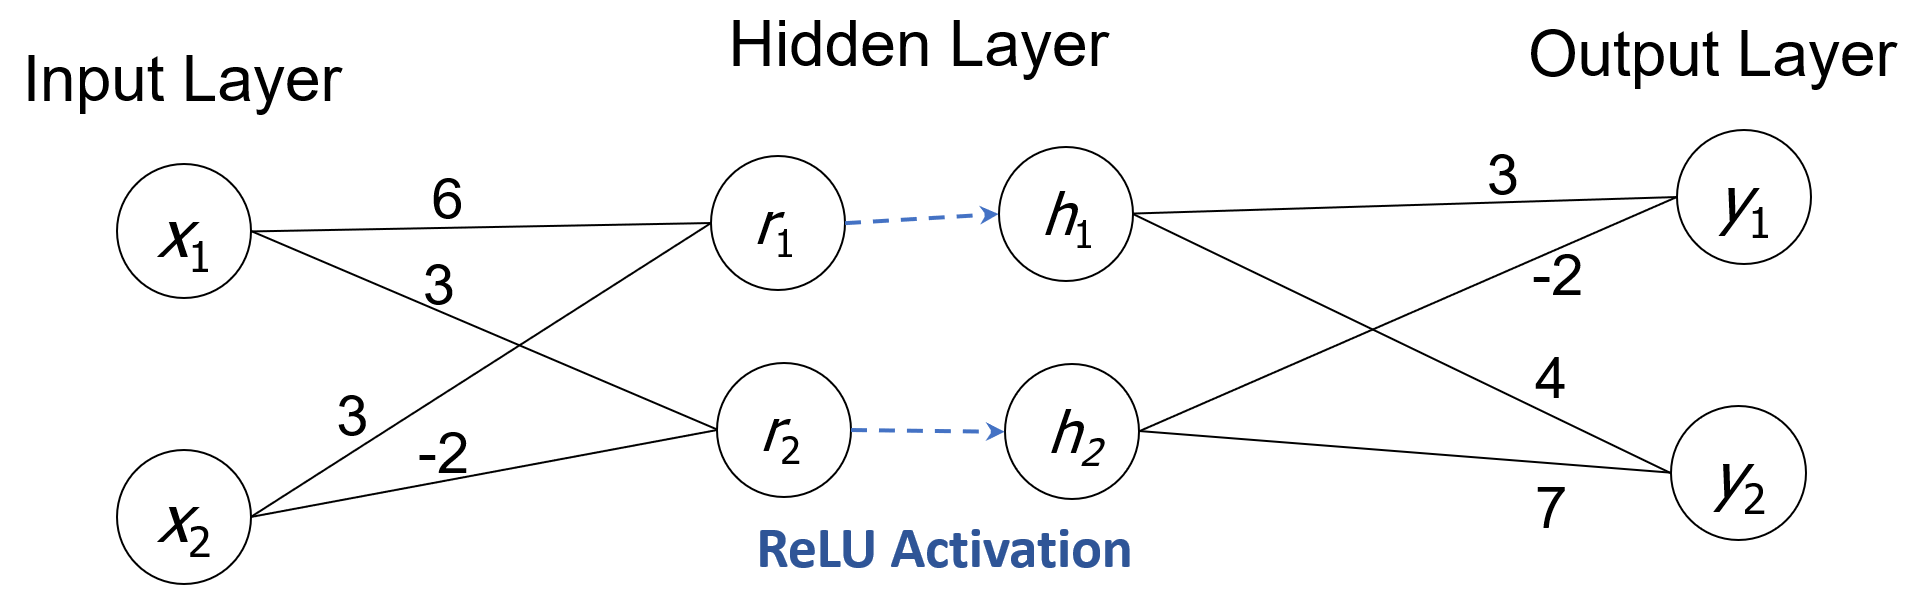
\includegraphics[width=0.8\linewidth]{images/robustnessVerification/q5.PNG}
	\caption{A neural network with one hidden layer with ReLU activation}
	\label{fig-q5}
\end{figure}

\begin{newquestion}{\textbf{5}~~}
\textbf{Lipschitz Continuity}

Given a neural network with one hidden layer with ReLU activation, shown as Figure~\ref{fig-q5}, please prove that the neural network is Lipschitz continuous. Please also calculate the Lipschitz constant of $y_1$ and $y_2$ w.r.t. $x_1$ and $x_2$.

\end{newquestion}



\begin{newquestion}{\textbf{6}~~}\label{q5}
\textbf{Reachability Problem}

Given a neural network with one hidden layer of ReLU activation (shown as Figure~\ref{fig-q5}), assume $x_1\in [3,6.5]$ and $x_2\in [2.5, 5.5]$, what is the output range of $y_1$ and $y_2$?

\begin{itemize}
    \item[1.] Please show how to solve the above reachability problem step by step using MILP/LP.
    
    \item[2.] Please show how to solve the above reachability problem step by step using global optimisation (i.e., DeepGO).
\end{itemize}
\end{newquestion}


\begin{newquestion}{\textbf{7}~~}
\textbf{Verification}

Based on the solution of Question~6,  show how to verify if $y_1\leq y_2$ given $x_1\in [3,6.5]$ and $x_2\in [2.5, 5.5]$?

\end{newquestion}
%%%%%%%%%%%%%%%%%%%%%%%%%%%%%%




\begin{newquestion}{\textbf{8}~~}
Understand the basic idea of adversarial training, and implement an adversarial training algorithm with different step size, number of steps, epoch, to see which hyper-parameter setting can achieve the best balance between performance and running time.  
\end{newquestion}



\begin{newquestion}{\textbf{9}~~}
Does adversarial training compromise the model's  clean accuracy? If so, how to mitigate it?  
\end{newquestion}



\begin{newquestion}{\textbf{10}~~}
Explore different assumptions on the distribution of random weights of DNNs, and understand which assumption is more reasonable in the PAC Bayesian theoretical framework. 
\end{newquestion}



\begin{newquestion}{\textbf{11}~~}
Figure out other technologies to improve generalisation performance of DNNs. 
\end{newquestion}